

	
% LaTeXar con :
%  pdflatex notebook.tex
% o bien,
%  latex notebook.dvi
%  dvipdfm notebook.dvi
%
%	" The PDF file may contain up to 25 pages of reference material, single-sided,
%   letter or A4 size, with text and illustrations readable by a person with
%   correctable eyesight without magnification from a distance of 1/2 meter. "
%
\documentclass[10pt,landscape,twocolumn,a4paper,notitlepage]{article}
\usepackage{hyperref}
\usepackage[spanish, activeacute]{babel}
\usepackage[utf8]{inputenc}
\usepackage{fancyhdr}
\usepackage{lastpage}
\usepackage{listings}
\usepackage{amssymb}
\usepackage[usenames,dvipsnames]{color}
\usepackage{graphicx}
\usepackage{wrapfig}



%%% Margenes
\setlength{\columnsep}{0.25in}    % default=10pt
\setlength{\columnseprule}{0.5pt}    % default=0pt (no line)
 
\addtolength{\textheight}{2.35in}
\addtolength{\topmargin}{-0.9in}     % ~ -0.5 del incremento anterior
 
\addtolength{\textwidth}{1.1in}
\addtolength{\oddsidemargin}{-0.55in} % -0.5 del incremento anterior
 
\setlength{\headsep}{0.08in}
\setlength{\parskip}{0in}
\setlength{\headheight}{15pt}
\setlength{\parindent}{0mm}
 
%%% Encabezado y pie de pagina
\pagestyle{fancy}
\fancyhead[LO]{\leftmark\ -\ \rightmark}
\fancyhead[C]{\textbf{\title}}
\fancyhead[RO]{P\'agina \thepage\ de \pageref{LastPage}}
\renewcommand{\headrulewidth}{0.4pt}
\fancyfoot{}
\definecolor{darkblue}{rgb}{0,0,0.4}
%%% Configuracion de Listings
\lstloadlanguages{C++}
\lstnewenvironment{code}
	{%\lstset{	numbers=none, frame=lines, basicstyle=\small\ttfamily, }%
	 \csname lst@SetFirstLabel\endcsname}
	{\csname lst@SaveFirstLabel\endcsname}
\lstset{% general command to set parameter(s)
	language=C++, basicstyle=\small\ttfamily, keywordstyle=\slshape,
	emph=[1]{tipo,usa}, emphstyle={[1]\sffamily\bfseries},
	morekeywords={tint,forn,forsn},
	basewidth={0.47em,0.40em},
	columns=fixed, fontadjust, resetmargins, xrightmargin=5pt, xleftmargin=15pt,
	flexiblecolumns=false, tabsize=2, breaklines,	breakatwhitespace=false, extendedchars=true,
	numbers=left, numberstyle=\tiny, stepnumber=1, numbersep=9pt,
	frame=l, framesep=3pt,
    basicstyle=\ttfamily,
    keywordstyle=\color{darkblue}\ttfamily,
    stringstyle=\color{magenta}\ttfamily,
    commentstyle=\color{RedOrange}\ttfamily,
    morecomment=[l][\color{OliveGreen}]{\#}
}

\lstdefinestyle{C++}{
	language=C++, basicstyle=\small\ttfamily, keywordstyle=\slshape,
	emph=[1]{tipo,usa}, emphstyle={[1]\sffamily\bfseries},
	morekeywords={tint,forn,forsn},
	basewidth={0.47em,0.40em},
	columns=fixed, fontadjust, resetmargins, xrightmargin=5pt, xleftmargin=15pt,
	flexiblecolumns=false, tabsize=2, breaklines,	breakatwhitespace=false, extendedchars=true,
	numbers=left, numberstyle=\tiny, stepnumber=1, numbersep=9pt,
	frame=l, framesep=3pt,
    basicstyle=\ttfamily,
    keywordstyle=\color{darkblue}\ttfamily,
    stringstyle=\color{magenta}\ttfamily,
    commentstyle=\color{RedOrange}\ttfamily,
    morecomment=[l][\color{OliveGreen}]{\#}
}
 
%%% Macros
\def\nbtitle#1{\begin{Large}\begin{center}\textbf{#1}\end{center}\end{Large}}
\def\nbsection#1{\section{#1}}
\def\nbsubsection#1{\subsection{#1}}
\def\nbcoment#1{\begin{small}\textbf{#1}\end{small}}
\newcommand{\comb}[2]{\left( \begin{array}{c} #1 \\ #2 \end{array}\right)}
\def\complexity#1{\texorpdfstring{$\mathcal{O}(#1)$}{O(#1)}}
 \newcommand\cppfile[2][]{
\lstinputlisting[style=C++,linerange={#1}]{#2.cpp}
}
\begin{document}

\def\title{El Diego 2.0}
 
%\begin{wrapfigure}{l}{0pt}
%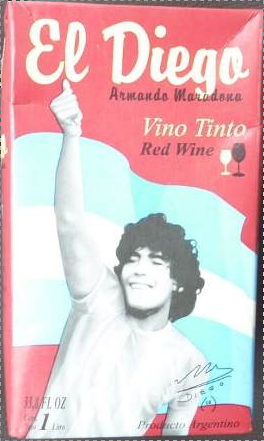
\includegraphics[width=2cm]{fotodiego}
%\end{wrapfigure}


\begin{center}
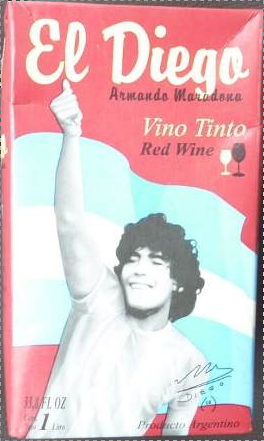
\includegraphics[width=5cm]{fotodiego}
\end{center}
\tableofcontents
\newpage
 
%%% El texto propiamente dicho
\section{Algoritmos}
\textbf{\#include $<$algorithm$>$ \#include $<$numeric$>$ \\}
\begin{tabular}{|l|l|p{5.4cm}|} \hline
\textbf{Algo} & \textbf{Params} &  \textbf{Funcion} \\  \hline
%swap & e1, e2 &  da vuelta e1,e2 & $1$\\\hline
sort, stable\_sort & f, l &  ordena el intervalo \\  \hline
%is\_sorted & f, l &  \textit{bool} si esta ordenado \\  \hline
nth\_element & f, nth, l & \textit{void} ordena el n-esimo, y \\ && particiona el resto \\  \hline
fill, fill\_n & f, l / n, elem & \textit{void} llena [f, l) o [f, \\ && f+n) con elem \\  \hline
lower\_bound, upper\_bound & f, l, elem & \textit{it} al primer / ultimo donde se \\ && puede insertar elem para que\\ && quede ordenada \\  \hline
binary\_search & f, l, elem & \textit{bool} esta elem en [f, l) \\  \hline
copy & f, l, resul & hace resul+$i$=f+$i$ $\forall i$ \\  \hline
find, find\_if, find\_first\_of & f, l, elem & \textit{it} encuentra i $\in$[f,l) tq. i$=$elem, \\ & / pred / f2, l2 & pred(i), i$\in$[f2,l2)\\\hline
count, count\_if & f, l, elem/pred & cuenta elem, pred(i)\\\hline
search & f, l, f2, l2 & busca [f2,l2) $\in$ [f,l)\\\hline
replace, replace\_if & f, l, old & cambia old / pred(i) por new \\ & / pred, new &\\\hline
reverse & f, l & da vuelta\\\hline
partition, stable\_partition & f, l, pred & pred(i) ad, !pred(i) atras\\\hline
%min, max & e1, e2 & men / may & $1$\\\hline
min\_element, max\_element & f, l, [comp] & \textit{it} min, max de [f,l]\\\hline
lexicographical\_compare & f1,l1,f2,l2 & \textit{bool} con [f1,l1]<[f2,l2]\\\hline
next/prev\_permutation & f,l & deja en [f,l) la perm sig, ant\\\hline
set\_intersection, & f1, l1, f2, l2, res & [res, $\ldots$) la op. de conj\\
set\_difference, set\_union, & & \\
set\_symmetric\_difference, & &\\\hline
push\_heap, pop\_heap, & f, l, e / e / & mete/saca e en heap [f,l), \\
make\_heap & & hace un heap de [f,l)\\\hline
is\_heap & f,l & \textit{bool} es [f,l) un heap\\\hline
accumulate & f,l,i,[op] & \textit{T} $=$ $\sum$/oper de [f,l)\\\hline
inner\_product & f1, l1, f2, i & \textit{T} $=$ i $+$ [f1, l1) . [f2, $\ldots$ )\\\hline
partial\_sum & f, l, r, [op] & r+i = $\sum$/oper de [f,f+i] $\forall i \in$[f,l)\\\hline
%power & e, i, op & \textit{T} = $e^{n}$\\\hline
\_\_builtin\_ffs& unsigned int x & Pos. del primer 1 desde la derecha\\\hline
\_\_builtin\_clz & unsigned int x & Cant. de ceros desde la izquierda.\\\hline
\_\_builtin\_ctz & unsigned int x & Cant. de ceros desde la derecha.\\\hline
\_\_builtin\_popcount & unsigned int x & Cant. de 1’s en x.\\\hline
\_\_builtin\_parity & unsigned int x & 1 si x es par, 0 si es impar.\\\hline
\end{tabular}


\section{Estructuras}
\subsection{RMQ (static)}
Dado un arreglo y una operación asociativa idempotente, get(i, j) opera sobre el rango [i, j). Restricción: LVL $\ge$ 2*ceil(logn); Usar [ ] para llenar arreglo y luego build().
\cppfile{estructuras/rmq.static}
\subsection{RMQ (dynamic)}
Dado un arreglo y una operación asociativa con neutro, get(i, j) opera sobre el rango [i, j).
\cppfile{estructuras/rmq.dynamic}
\subsection{Fenwick Tree}
For 2D threat each column as a Fenwick tree, by adding a nested for in each operation
\cppfile{estructuras/fenwick}
\subsection{Union Find}
\cppfile{estructuras/union.find}
\subsection{Disjoint Intervals}
\cppfile{estructuras/disjoint.intervals}
\subsection{RMQ (2D)}
\cppfile{estructuras/rmq.2d}
\subsection{Big Int}
\cppfile{estructuras/bigint}
\subsection{Modnum}
\cppfile{estructuras/mnum}
\subsection{Bittrie}
\cppfile{estructuras/bitrie}

\section{Strings}
\subsection{Trie}
\cppfile{string/trie}
\subsection{Suffix Array}
\cppfile[-34]{string/suffix.array}
\subsection{String Matching With Suffix Array}
\cppfile[37-58]{string/suffix.array}
\subsection{LCP (Longest Common Prefix)}
\cppfile[60-75]{string/suffix.array}
\section{Geometría}
\#define EPS 1e-9
\subsection{Punto}
\cppfile{geometria/pto}
\subsection{Line}
\cppfile{geometria/line}
\subsection{Segment}
\cppfile{geometria/segm}
\subsection{Rectangle}
\cppfile{geometria/rect}
\subsection{Polygon Area}
\cppfile{geometria/area}
\subsection{Circle}
\cppfile{geometria/circle}
\subsection{Point in Poly}
\cppfile{geometria/point.in.poly}
\subsection{Convex Check CHECK}
\cppfile{geometria/convex.check}
\subsection{Convex Hull}
\cppfile{geometria/convex.hull}
\subsection{Cut Polygon}
\cppfile{geometria/cut.polygon}
\subsection{Bresenham}
\cppfile{geometria/bresenham}
\subsection{Rotate Matrix}
\cppfile{geometria/rotate}
\section{Math}
\subsection{GCD}
\begin{code}
tipo gcd(tipo a, tipo b){return a?gcd(b %a, a):b;}
\end{code}
\subsection{LCM}
\begin{code}
tipo lcm(tipo a, tipo b){return a*b/gcd(a, b);}
\end{code}
\subsection{Simpson}
\cppfile{math/simpson}
\subsection{Fraction}
\cppfile{math/frac}
\subsection{Polinomio}
\cppfile{math/polinomio}
\section{Grafos}
\subsection{Dijkstra}
\begin{code}
#define INF 1e9
int N;
#define MAX_V 250001
vector<ii> G[MAX_V];
//To add an edge use
#define add(a, b, w) G[a].pb(mkp(w, b))

ll dijkstra(int s, int t){//O(|E| log |V|)
	priority_queue<ii, vector<ii>, greater<ii> > Q;
	vector<ll> dist(N, INF); vector<int> dad(N, -1);
	Q.push(mkp(0, s)); dist[s] = 0;
	while(sz(Q)){
		ii p = Q.top(); Q.pop();
		if(p.snd == t) break;
		forall(it, G[p.snd])
			if(dist[p.snd]+it->first < dist[it->snd]){
				dist[it->snd] = dist[p.snd] + it->fst;
				dad[it->snd] = p.snd;
				Q.push(mkp(dist[it->snd], it->snd));
			}
	}
	return dist[t];
	if(dist[t]<INF)//path generator
		for(int i=t; i!=-1; i=dad[i])
			printf("%d%c", i, (i==s?'\n':' '));
}
\end{code}
\subsection{Bellman-Ford}
\begin{code}
vector<ii> G[MAX_N];//ady. list with pairs (weight, dst)
int dist[MAX_N];
void bford(int src){//O(VE)
	dist[src]=0;
	forn(i, N-1) forn(j, N) if(dist[j]!=INF) forall(it, G[j])
		dist[it->snd]=min(dist[it->snd], dist[j]+it->fst);
}

bool hasNegCycle(){
	forn(j, N) if(dist[j]!=INF) forall(it, G[j])
		if(dist[it->snd]>dist[j]+it->fst) return true;
	//inside if: all points reachable from it->snd will have -INF distance(do bfs)
	return false;
}
\end{code}
\subsection{Floyd-Warshall}
G[i][j] contains weight of edge (i, j) or INF
G[i][i]=0
\begin{code}
int G[MAX_N][MAX_N];
void floyd(){//O(N^3)
forn(k, N) forn(i, N) if(G[i][k]!=INF) forn(j, N) if(G[k][j]!=INF)
	G[i][j]=min(G[i][j], G[i][k]+G[k][j]);
}
bool inNegCycle(int v){
	return G[v][v]<0;}
//checks if there's a neg. cycle in path from a to b
bool hasNegCycle(int a, int b){
	forn(i, N) if(G[a][i]!=INF && G[i][i]<0 && G[i][b]!=INF)
		return true;
	return false;
}
\end{code}
\subsection{2-SAT + Tarjan SCC}
We have a vertex representing a var and other for his negation.
Every edge stored in G represents an implication. To add an equation of the form a||b, use addor(a, b)
MAX=max cant var, n=cant var
\begin{code}
#define addor(a, b) (G[neg(a)].pb(b), G[neg(b)].pb(a)) 
vector<int> G[MAX*2];
//idx[i]=index assigned in the dfs
//lw[i]=lowest index(closer from the root) reachable from i
int lw[MAX*2], idx[MAX*2], qidx;
stack<int> q;
int qcmp, cmp[MAX*2];
//verdad[cmp[i]]=valor de la variable i
bool verdad[MAX*2+1];

int neg(int x) { return x>=n? x-n : x+n;}
void tjn(int v){
	lw[v]=idx[v]=++qidx;
	q.push(v), cmp[v]=-2;
	forall(it, G[v]){
		if(!idx[*it] || cmp[*it]==-2){
			if(!idx[*it]) tjn(*it);
			lw[v]=min(lw[v], lw[*it]);
		}
	}
	if(lw[v]==idx[v]){
		qcmp++;
		int x;
		do{x=q.top(); q.pop(); cmp[x]=qcmp;}while(x!=v);
		verdad[qcmp]=(cmp[neg(v)]<0);
	}
}
//remember to CLEAR G!!!
bool satisf(){//O(n)
	memset(idx, 0, sizeof(idx)), qidx=0;
	memset(cmp, -1, sizeof(cmp)), qcmp=0;
	forn(i, n){
		if(!idx[i]) tjn(i);
		if(!idx[neg(i)]) tjn(neg(i));
	}
	forn(i, n) if(cmp[i]==cmp[neg(i)]) return false;
	return true;
}
\end{code}
\subsection{Articulation Points}
\begin{code}
int N;
vector<int> G[1000000];
//V[i]=node number(if visited), L[i]= lowest V[i] reachable from i
int qV, V[1000000], L[1000000], P[1000000];
void dfs(int v, int f){
	L[v]=V[v]=++qV;
	forall(it, G[v])
		if(!V[*it]){
			dfs(*it, v);
			L[v] = min(L[v], L[*it]);
			P[v]+= L[*it]>=V[v];
		}
		else if(*it!=f)
			L[v]=min(L[v], V[*it]);
}
int cantart(){ //O(n)
	qV=0;
	zero(V), zero(P);
	dfs(1, 0); P[1]--;
	int q=0;
	forn(i, N) if(P[i]) q++;
return q;
}
\end{code}
\subsection{LCA + Climb}
\begin{code}
LCA
#define POT2(x) (1<<(x))
//f[v][k] holds the 2^k father of v
//L[v] holds the level of v
int N, f[100001][20], L[100001];
void build(){//f[i][0] must be filled previously, O(nlgn)
	forn(k, 20-1) forn(i, N) f[i][k+1]=f[f[i][k]][k];}
int lg(int x){//=floor(log2(x))
	int i;
	for (i=0;(1<<i)<=x;i++) ;
	return i-1;
}
int climb(int a, int d){//O(lgn)
	if(!d) return a;
	dforn(i, lg(L[a])+1)
		if(POT2(i)<=d)
			a=f[a][i], d-=POT2(i);
    return a;
}
int lca(int a, int b){//O(lgn)
	if(L[a]<L[b]) swap(a, b);
	a=climb(a, L[a]-L[b]);
	if(a==b) return a;
	dforn(i, lg(L[a])+1)
		if(f[a][i]!=f[b][i])
			a=f[a][i], b=f[b][i];
	return f[a][0];
}
\end{code}
\section{Network Flow}
\subsection{Edmonds Karp’s}
\begin{code}
#define MAX_V 1000
#define INF 1e9
//special nodes
#define SRC 0
#define SNK 1
map<int, int> G[MAX_V];//limpiar esto
//To add an edge use
#define add(a, b, w) G[a][b]=w
int f, p[MAX_V];
void augment(int v, int minE){
	if(v==SRC) f=minE;
	else if(p[v]!=-1){
		augment(p[v], min(minE, G[p[v]][v]));
		G[p[v]][v]-=f, G[v][p[v]]+=f;
	}
}
ll maxflow(){//O(VE^2)
	ll Mf=0;
	do{
		f=0;
		char used[MAX_V]; queue<int> q; q.push(SRC);
		zero(used), memset(p, -1, sizeof(p));
		while(sz(q)){
			int u=q.front(); q.pop();
			if(u==SNK) break;
			forall(it, G[u])
				if(it->snd>0 && !used[it->fst])
					used[it->fst]=true, q.push(it->fst), p[it->fst]=u;
		}
		augment(SNK, INF);
		Mf+=f;
	}while(f);
	return Mf;
}
\end{code}
\subsection{Push-Relabel}
\begin{code}
#define MAX_V 1000
int N;//valid nodes are [0...N-1]
#define INF 1e9
//special nodes
#define SRC 0
#define SNK 1
map<int, int> G[MAX_V];
//To add an edge use
#define add(a, b, w) G[a][b]=w
ll excess[MAX_V];
int height[MAX_V], active[MAX_V], count[2*MAX_V+1];
queue<int> Q;
void enqueue(int v) { 
	if (!active[v] && excess[v] > 0) active[v]=true, Q.push(v); }
void push(int a, int b) {
	int amt = min(excess[a], ll(G[a][b]));
	if(height[a] <= height[b] || amt == 0) return;
	G[a][b]-=amt, G[b][a]+=amt;
	excess[b] += amt, excess[a] -= amt;
	enqueue(b);
}
void gap(int k) {
	forn(v, N){
		if (height[v] < k) continue;
		count[height[v]]--;
		height[v] = max(height[v], N+1);
		count[height[v]]++;
		enqueue(v);
	}
}
void relabel(int v) {
	count[height[v]]--;
	height[v] = 2*N;
	forall(it, G[v])
		if(it->snd)
			height[v] = min(height[v], height[it->fst] + 1);
	count[height[v]]++;
	enqueue(v);
}
ll maxflow() {//O(V^3)
	zero(height), zero(active), zero(count), zero(excess);
	count[0] = N-1;
	count[N] = 1;
	height[SRC] = N;
	active[SRC] = active[SNK] = true;
	forall(it, G[SRC]){
		excess[SRC] += it->snd;
		push(SRC, it->fst);
	}
	while(sz(Q)) {
		int v = Q.front(); Q.pop();
		active[v]=false;
	forall(it, G[v]) push(v, it->fst);
	if(excess[v] > 0) 
		count[height[v]] == 1? gap(height[v]):relabel(v);
	}
	ll mf=0;
	forall(it, G[SRC]) mf+=G[it->fst][SRC];
	return mf;
}
\end{code}
\section{Ayudamemoria}
\subsection*{Límites}
\begin{code}
#include <climits> //INT_MIN, LONG_MAX, ULLONG_MAX, etc.
\end{code}
\subsection*{Cant. decimales}
\begin{code}
#include <iomanip>
cout << setprecision(2) << fixed;
\end{code}
\subsection*{Rellenar con espacios(para justificar)}
\begin{code}
#include <iomanip>
cout << setfill(' ') << setw(3) << 2 << endl;
\end{code}
\subsection*{Leer hasta fin de línea}
\begin{code}
#include <sstream>
//hacer cin.ignore() antes de getline()
while(getline(cin, line)){
   	 istringstream is(line);
   	 while(is >> X)
   		 cout << X << " ";
   	 cout << endl;
}
\end{code}
\subsection*{Aleatorios}
\begin{code}
#define RAND(a, b) (rand()%(b-a+1)+a)
srand(time(NULL));
\end{code}
\subsection*{Muahaha}
\begin{code}
#include <climits> //INT_MIN, LONG_MAX, ULLONG_MAX, etc.
\end{code}
\subsection*{Límites}
\begin{code}
#include <signal.h>
void divzero(int p){
	while(true);}
void segm(int p){
	exit(0);}
//in main
signal(SIGFPE, divzero);
signal(SIGSEGV, segm);
\end{code}
\subsection*{Mejorar velocidad}
\begin{code}
ios::sync_with_stdio(false);
\end{code}
\subsection*{Leer del teclado}
\begin{code}
freopen("/dev/tty", "a", stdin);
\end{code}
\subsection*{File setup}
\begin{code}
//tambien se pueden usar comas: {a, x, m, l}
for i in {a..k}; do cp template.cpp $i.cpp; touch $i.in; done
\end{code}
\end{document}
